\Subhead{2.8.1}{Образование разрывов. Ударные волны}

Нелинейность означает, что локальная скорость распространения зависит от возмущения. Для одномерной простой волны малой, но конечной акустической амплитуды
\begin{equation}
 u_t+(c_0+\beta u)u_x=0,\qquad
 \beta=1+\frac{B}{2A}.
\end{equation}
$u$ — скорость частиц, $A=\rho_0c_0^2$, $B=\rho_0^2(\partial^2p/\partial\rho^2)_s$ — коэффициенты разложения уравнения состояния. Для идеального газа $\beta=(\gamma_{\rm ad}+1)/2$. Характеристики задаются $u=u_0(\xi)$, $x=\xi+[c_0+\beta u_0(\xi)]t$; отсюда
\begin{equation}
 u_x=\frac{u'_0(\xi)}{1+\beta t u'_0(\xi)},\qquad
 t_{\rm sh}=-\frac1{\min_\xi[\beta u'_0(\xi)]}
\end{equation}
при отрицательном минимуме. Сжатые участки догоняют разреженные, профиль становится всё круче. После обращения знаменателя в нуль многозначная формальная характеристическая кривая не является физическим решением: возникает ударный фронт.

В сопутствующем времени $\tau=t-x/c_0$, на расстояниях медленного изменения профиля
\begin{equation}
 u_x-\frac{\beta}{c_0^2}u u_\tau=0.
\end{equation}
Для $u(0,\tau)=u_a\sin\omega\tau$ разрыв впервые формируется на $x_{\rm sh}=c_0^2/(\beta\omega u_a)$. Ударная волна определяется также сохранением массы, импульса и энергии через фронт и условием роста энтропии; простой переворот профиля не заменяет этих условий.
\begin{center}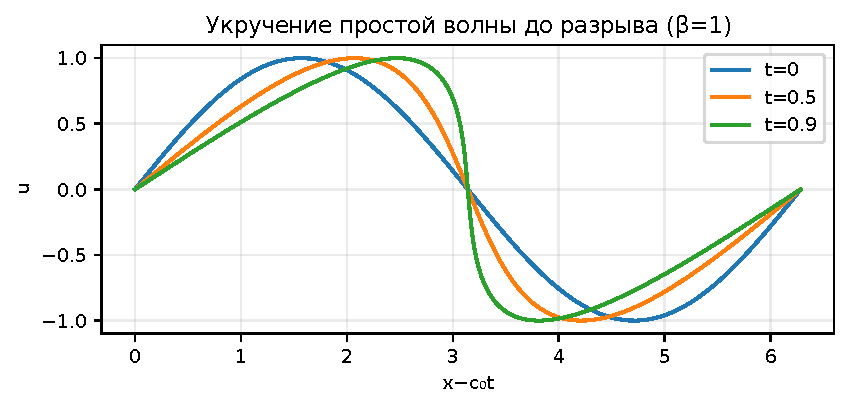
\includegraphics[width=0.8\linewidth]{figures/shock.pdf}\end{center}

